\subsubsection{\texttt{RF-1}: autenticación de usuarios y visualización de sus recursos asociados}
\label{subsec:rf1}

Este requisito establece la necesidad de que los usuarios de \textit{VSCode4Teaching} puedan autenticarse en la aplicación web para visualizar únicamente sus recursos legítimamente accesibles. Cabe dividir este requisito en dos partes: la autenticación (\texttt{RF-1.1}) y la visualización de los cursos asociados (\texttt{RF-1.2}).

El requisito \texttt{RF-1.1} establece la necesidad de que los usuarios puedan iniciar sesión para autenticarse utilizando su nombre de usuario y contraseña asociada, garantizando así que son quien dicen ser. Para ello, la aplicación web introduce un formulario que permite a los usuarios introducir las credenciales que ya venían utilizando para la verificación de su identidad en la extensión para Visual Studio Code en versiones anteriores, tal como refleja la \referenciaFigura{fig:reqf1-1}.

\begin{figure}[ht]
    \centering
    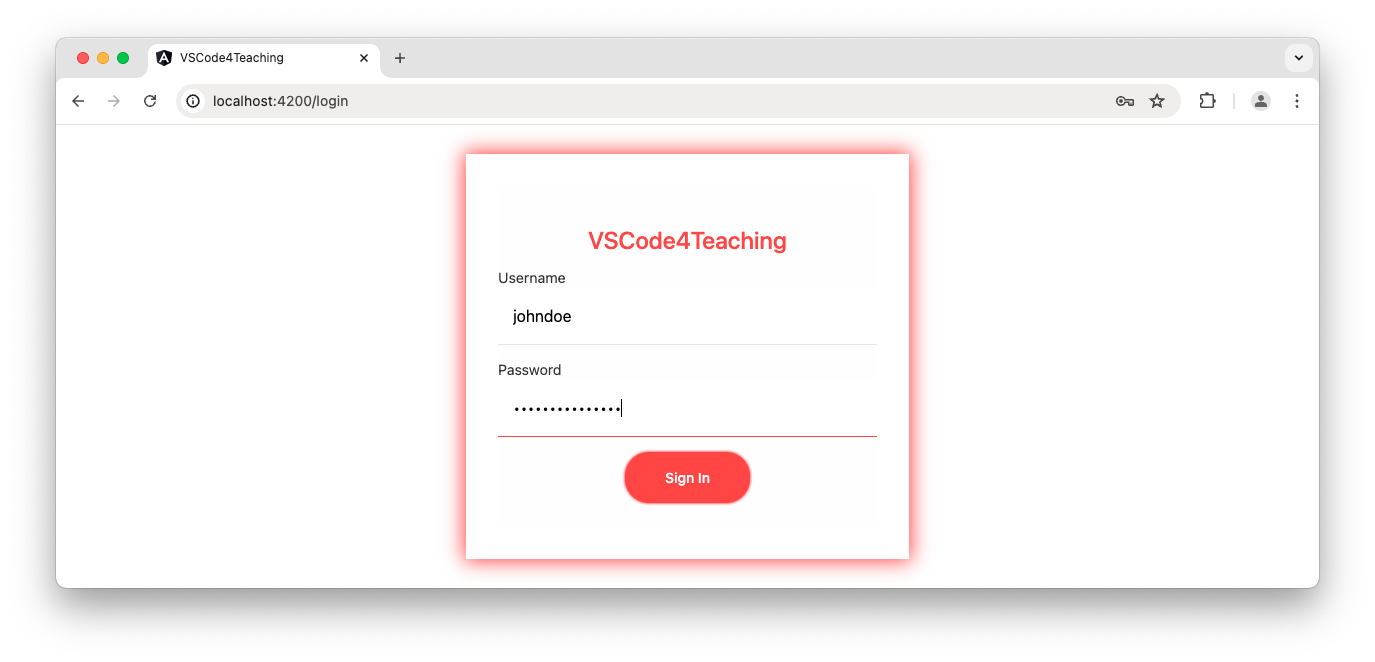
\includegraphics[width=\textwidth]{imagenes/utilizadas/4-3-implementacion/rf1-1.png}
    \caption{Formulario de inicio de sesión para usuarios registrados en la aplicación web.}
    \label{fig:reqf1-1}
\end{figure}

Una vez cumplimentado, las credenciales se envían al servidor y, en caso de ratificarse su validez, se genera un \textit{token} relativo a la sesión activa del usuario que queda almacenado en el contexto de la pestaña activa mediante el uso del \textit{sessionStorage}, que es un almacenamiento del navegador que permite almacenar pares clave-valor que persisten únicamente al contexto de la página que los crea (por contraposición con el \textit{localStorage}, que persiste a la finalización de la sesión activa salvo que se cierre la sesión ex profeso).

Por otro lado, el requisito \texttt{RF-1.2} especifica que los usuarios autenticados deben poder visualizar los recursos que tenga asociados a su cuenta. Para ello, una vez que los usuarios inician sesión en la aplicación, visualizan una pantalla de inicio que muestra los cursos de los que forman parte (\referenciaFigura{fig:reqf1-2}) que varía según el rol: mientras que los estudiantes tienen un botón para acceder a la pantalla en la que comienzan a realizar ejercicios (\referenciaConTT{subsec:rf9}{RF-9}), los docentes acceden a una interfaz (\referenciaFigura{fig:reqf1-3}) en la que pueden visualizar los ejercicios de los que dispone el curso con información básica sobre el progreso de cada uno y, además, crear nuevos ejercicios (\referenciaConTT{subsec:rf2}{RF-2}), gestionar los alumnos matriculados (\referenciaConTT{subsec:rf6}{RF-6}) y compartir el curso (\referenciaConTT{subsec:rf7}{RF-7}).

\begin{figure}[ht]
    \centering
    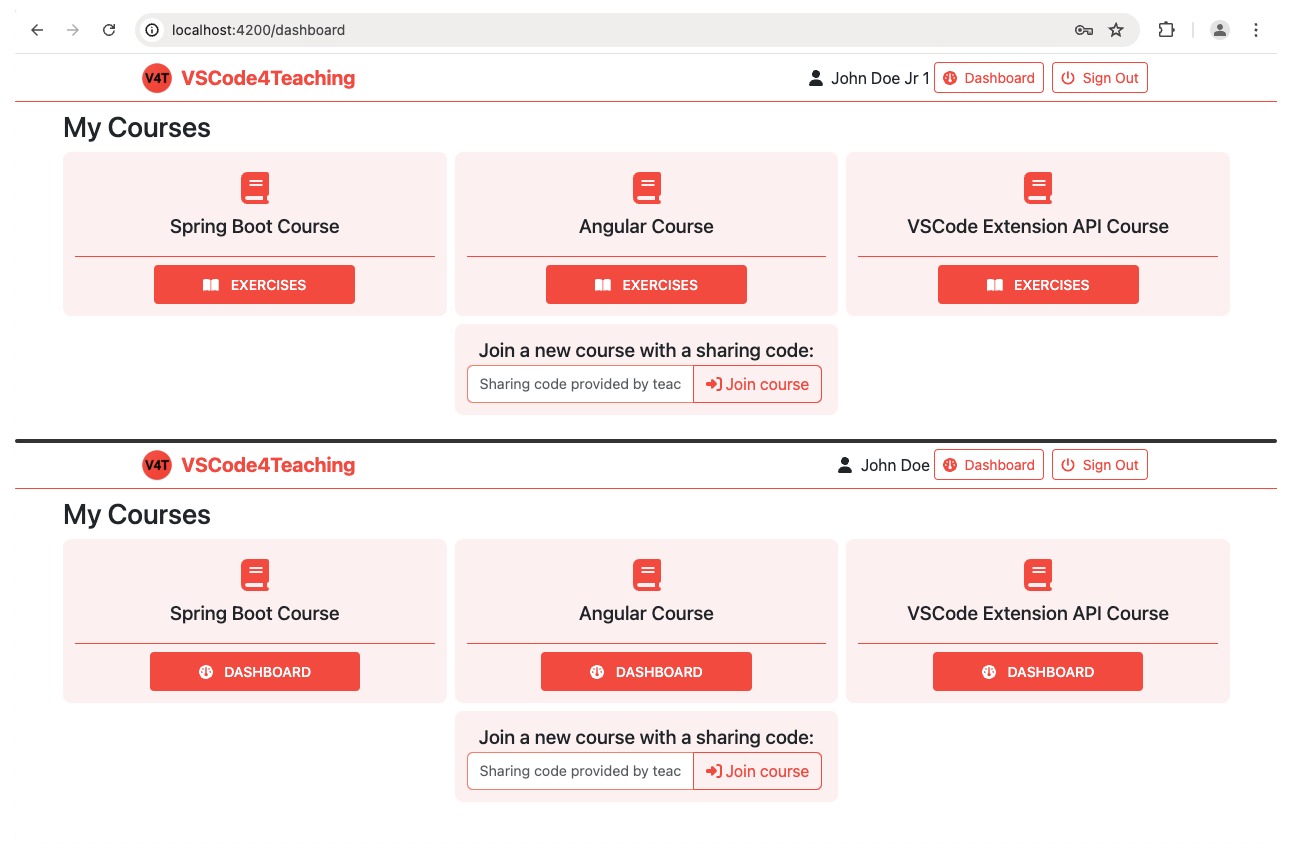
\includegraphics[width=\textwidth]{imagenes/utilizadas/4-3-implementacion/rf1-2.png}
    \caption{Pantalla de inicio para usuarios autenticados, tanto estudiantes (arriba) como docentes (abajo).}
    \label{fig:reqf1-2}
\end{figure}

\begin{figure}[ht]
    \centering
    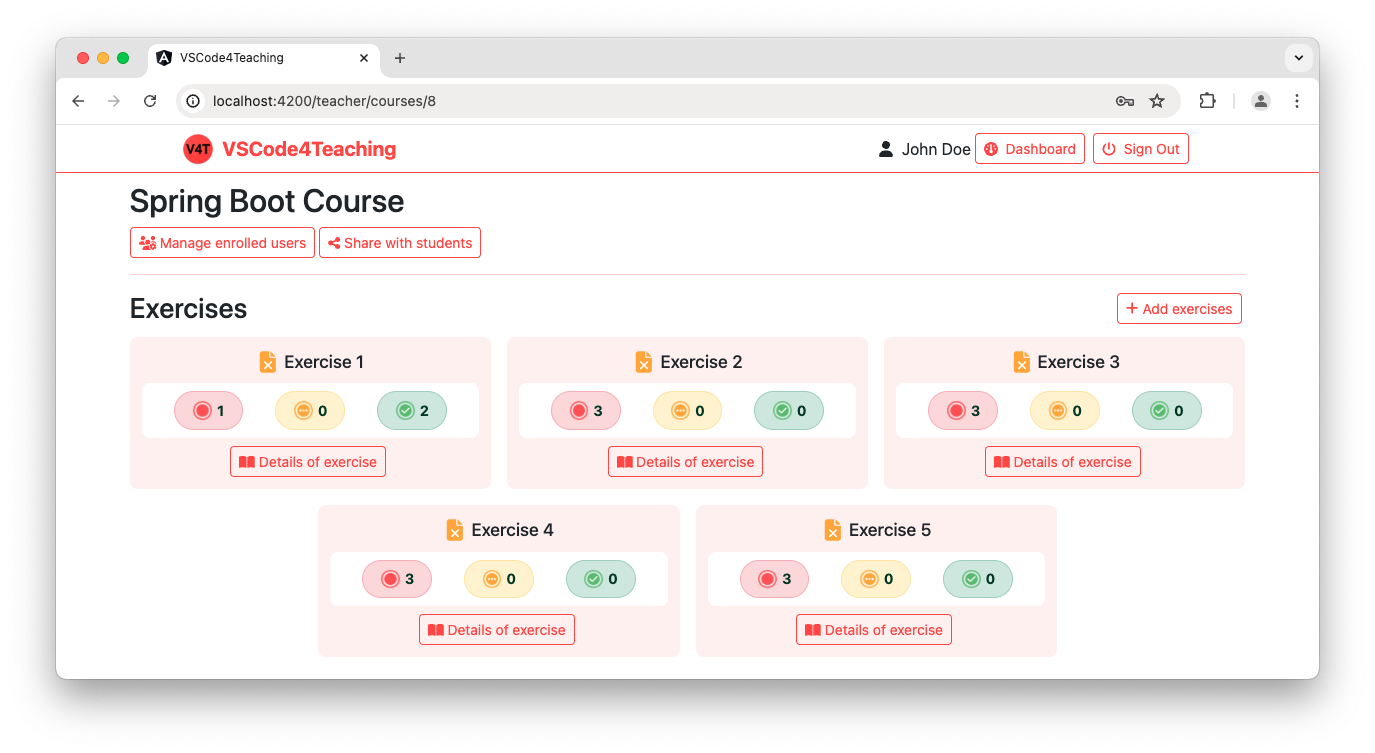
\includegraphics[width=\textwidth]{imagenes/utilizadas/4-3-implementacion/rf1-3.png}
    \caption{Interfaz principal para docentes acerca de cada uno de sus cursos impartidos.}
    \label{fig:reqf1-3}
\end{figure}
